
\documentclass[final]{beamer}

\usepackage[scale=1.24]{beamerposter} % Use the beamerposter package for laying out the poster
\usepackage{float}
\usepackage{times}
\usepackage{latexsym}
\usepackage{amsmath}
\usepackage{tikz, pgfplots}
\usetheme{confposter} % Use the confposter theme supplied with this template

\setbeamercolor{block title}{fg=ngreen,bg=white} % Colors of the block titles
\setbeamercolor{block body}{fg=black,bg=white} % Colors of the body of blocks
\setbeamercolor{block alerted title}{fg=white,bg=dblue!70} % Colors of the highlighted block titles
\setbeamercolor{block alerted body}{fg=black,bg=dblue!10} % Colors of the body of highlighted blocks
% Many more colors are available for use in beamerthemeconfposter.sty

%-----------------------------------------------------------
% Define the column widths and overall poster size
% To set effective sepwid, onecolwid and twocolwid values, first choose how many columns you want and how much separation you want between columns
% In this template, the separation width chosen is 0.024 of the paper width and a 4-column layout
% onecolwid should therefore be (1-(# of columns+1)*sepwid)/# of columns e.g. (1-(4+1)*0.024)/4 = 0.22
% Set twocolwid to be (2*onecolwid)+sepwid = 0.464
% Set threecolwid to be (3*onecolwid)+2*sepwid = 0.708

\newlength{\sepwid}
\newlength{\onecolwid}
\newlength{\twocolwid}
\newlength{\threecolwid}
\setlength{\paperwidth}{48in} % A0 width: 46.8in
\setlength{\paperheight}{36in} % A0 height: 33.1in
\setlength{\sepwid}{0.024\paperwidth} % Separation width (white space) between columns
\setlength{\onecolwid}{0.22\paperwidth} % Width of one column
\setlength{\twocolwid}{0.464\paperwidth} % Width of two columns
\setlength{\threecolwid}{0.708\paperwidth} % Width of three columns
\setlength{\topmargin}{-0.5in} % Reduce the top margin size
%-----------------------------------------------------------

\usepackage{graphicx}  % Required for including images

\usepackage{booktabs} % Top and bottom rules for tables

%----------------------------------------------------------------------------------------
%	TITLE SECTION 
%----------------------------------------------------------------------------------------

\title{Data Mining \& Big Data: A URL Categorization System} % Poster title

\author{Montagner A., Viglianisi E.} % Author(s)

\institute{University of Trento, 2017} % Institution(s)

%----------------------------------------------------------------------------------------

\begin{document}

\addtobeamertemplate{block end}{}{\vspace*{2ex}} % White space under blocks
\addtobeamertemplate{block alerted end}{}{\vspace*{2ex}} % White space under highlighted (alert) blocks

\setlength{\belowcaptionskip}{2ex} % White space under figures
\setlength\belowdisplayshortskip{2ex} % White space under equations

\begin{frame}[t] % The whole poster is enclosed in one beamer frame

\begin{columns}[t] % The whole poster consists of three major columns, the second of which is split into two columns twice - the [t] option aligns each column's content to the top

\begin{column}{\sepwid}\end{column} % Empty spacer column

\begin{column}{\onecolwid} % The first column

%----------------------------------------------------------------------------------------
%	OBJECTIVES
%----------------------------------------------------------------------------------------

\begin{alertblock}{Objectives}
Project's objectives:
\begin{itemize}
\item Introduce URL Categorization problem.
\item Quick discussion on Topic Modeling algorithms.
\item Provide a linear (Data Mining approach) and a parallel solution (Big Data approach).
\item Show results for both solution.
\end{itemize}

\end{alertblock}

%----------------------------------------------------------------------------------------
%    URL CATEGORIZATION PROBLEM
%----------------------------------------------------------------------------------------

\begin{block}{URL Categorization Problem}

\noindent{{\bfseries STEP 1:}} 
	\begin{description}
    	\item [INPUT] - A dataset of geotagged URL in M\\ 
					  - A grid of sizes S1xS1 over M
		
		\item [OUTPUT] - Main topics for each cell of the grid $S1$x$S1$.\\
	\end{description}
		
\noindent{\bfseries STEP 2:}
\begin{description}
		\item [INPUT] - A grid of sizes S1xS1 over M, with main topics that were computed in the STEP1.\\
					  - A grid of sizes S2xS2 over M

					  
		\item [OUTPUT] - Main topics for each cell of the grid S2xS2.\\
	\end{description}	

\end{block}

%------------------------------------------------

\begin{figure}[h]
\center{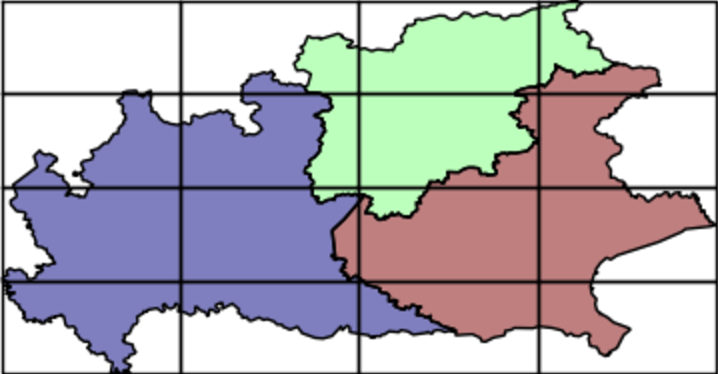
\includegraphics[width=\textwidth]{images/trentino}}
\center{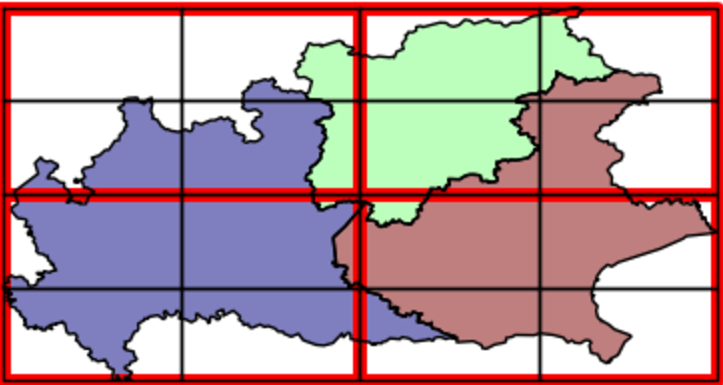
\includegraphics[width=\textwidth]{images/trentinored}}
	\caption{Example of grid division and grid scaling}
\end{figure}

%----------------------------------------------------------------------------------------

\end{column} % End of the first column

\begin{column}{\sepwid}\end{column} % Empty spacer column

\begin{column}{\twocolwid} % Begin a column which is two columns wide (column 2)

\begin{columns}[t,totalwidth=\twocolwid] % Split up the two columns wide column

\begin{column}{\onecolwid}\vspace{-.6in} % The first column within column 2 (column 2.1)

%----------------------------------------------------------------------------------------
%	MATERIALS
%----------------------------------------------------------------------------------------

\begin{block}{Topic Modeling algorithms}
\begin{itemize}
\item lda.update: exploits a method from Gensim library. Its updates an already trained model with new unseen corpus.

\item Top\_Topic Aggregation: Pre-compute once the LDA model of the entire map (global model), asking for a large number of topics. Then, computes the \emph{top\_topic distributions} of the corpus of each subcell. Finally, topic distributions of the subcells are merged to obtain the topic distribution of the entire cell. Allows to save time during the evaluation of top topics: top topics of the new cell are computed by summing together the resulting topics' weights of the already computed sub-cells, instead of iterating again over all the document of the area.

\end{itemize}


\end{block}

%----------------------------------------------------------------------------------------

\end{column} % End of column 2.1

\begin{column}{\onecolwid}\vspace{-.6in} % The second column within column 2 (column 2.2)

%----------------------------------------------------------------------------------------
%	DATA MINING
%----------------------------------------------------------------------------------------

\begin{block}{Data Mining solution}
Tests show both strong points and weaknesses of the proposed algorithms. \begin{itemize}
\item \emph{Top\_Topic Aggregation}: it is more suitable when the areas are large and every area contains a non negligible portion of the whole dataset.
\item \emph{lda\_update}: it is the best choice when small increases of the dimensions of the cells are taken in consideration, so that the model will be updated with few documents. \\[.6cm]

There is no single best way of solving this problem, but rather a combination of the two methods, depending on the required application. 
\end{itemize}    

\end{block}

%----------------------------------------------------------------------------------------

\end{column} % End of column 2.2

\end{columns} % End of the split of column 2 - any content after this will now take up 2 columns width

%----------------------------------------------------------------------------------------

\begin{columns}[t,totalwidth=\twocolwid] % Split up the two columns wide column again

\begin{column}{\onecolwid} % The first column within column 2 (column 2.1)

%----------------------------------------------------------------------------------------
%	BIG DATA
%----------------------------------------------------------------------------------------

\begin{block}{Big Data solution}

Since the other two algorithms are very difficult to parallelize, \emph{Top\_Topic Aggregation} is the most suitable for this approach because it does not need to maintain an updated shared object.

\begin{figure}[h]
	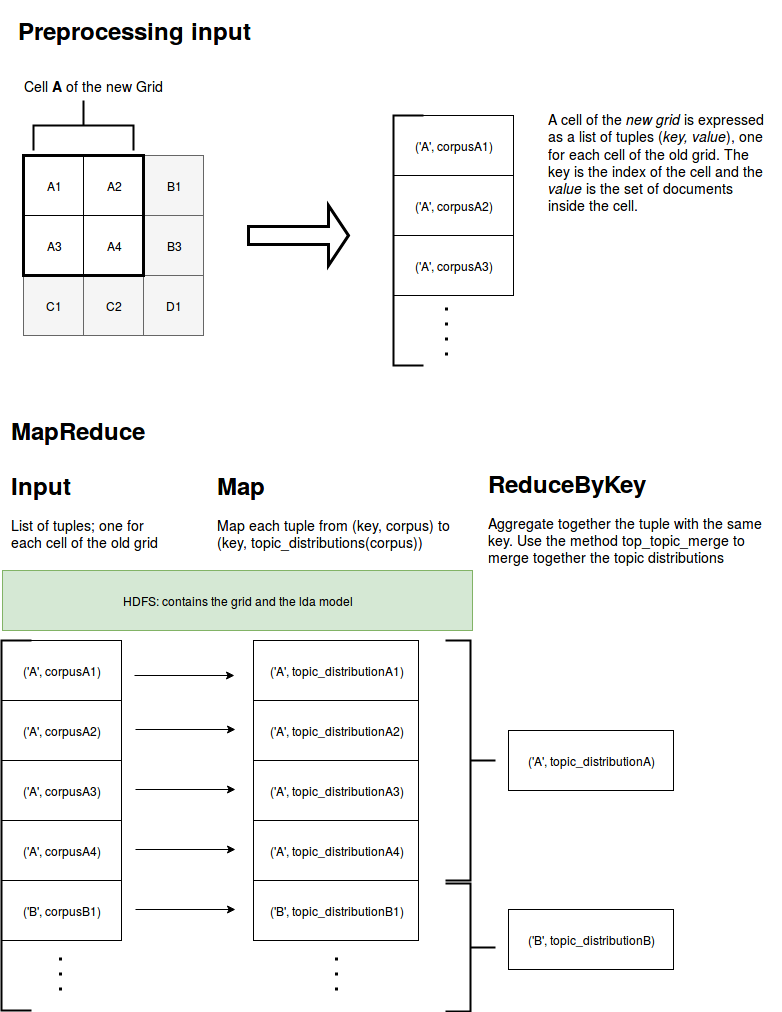
\includegraphics[scale=.9]{images/mapreduce}
	\caption{Mapreduce}
\end{figure}

\end{block}

%----------------------------------------------------------------------------------------

\end{column} % End of column 2.1

\begin{column}{\onecolwid} % The second column within column 2 (column 2.2)

%----------------------------------------------------------------------------------------
%	SPARK STREAMING
%----------------------------------------------------------------------------------------

\begin{block}{ Streaming Spark}

MapReduce algorithm is applied for each chunk of data (which spark obtains discretizing the stream) and, when the results for a chunk are ready, they are merged into to the topic distributions of the existing grid.

\begin{figure}[h]
	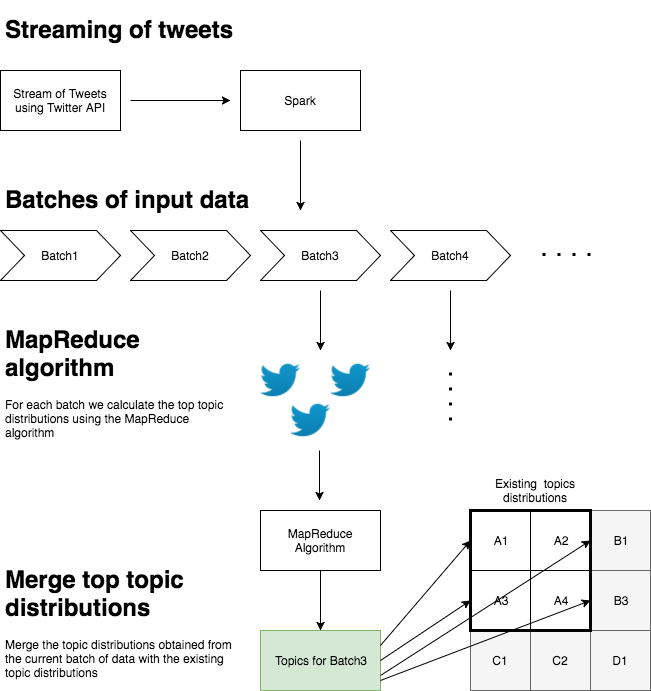
\includegraphics[]{images/streamingspark3}
	\caption{Spark Streaming}
\end{figure}

\end{block}

%----------------------------------------------------------------------------------------

\end{column} % End of column 2.2

\end{columns} % End of the split of column 2

\end{column} % End of the second column

\begin{column}{\sepwid}\end{column} % Empty spacer column

\begin{column}{\onecolwid} % The third column

%----------------------------------------------------------------------------------------
%	Results
%----------------------------------------------------------------------------------------

\begin{block}{Data Mining Results}

\begin{table}[]
\centering
\caption{My caption}
\label{my-label}
\begin{tabular}{@{}ccc@{}}
\toprule
\multicolumn{1}{l}{\textit{\textbf{Documents}}} & \textit{\textbf{Top Topic Aggr}} & \textit{\textbf{lda.update}} \\ \midrule
\textit{5056}                                   & \textit{6}                       & \textit{7}                                   \\
\textit{14329}                                  & \textit{10}                      & \textit{10}                                  \\
\textit{430}                                    & \textit{1}                       & \textit{3}                                   \\ \bottomrule
\end{tabular}
\end{table}

\end{block}


%----------------------------------------------------------------------------------------
%	DATA MINING RESULTS
%----------------------------------------------------------------------------------------



\begin{block}{Big Data Results}
\begin{tikzpicture}
\begin{axis}[
	height=25cm,
	width=24cm,
    title={Processed documents (thousands) per seconds},
    xlabel={},
    ylabel={},
    xmin=100, xmax=1000,
    ymin=70, ymax=3000,
    xtick={100,200,500,1000},
    ytick={100,200,400,800,1600,3000},
    legend pos=north west,
    ymajorgrids=true,
    grid style=dashed,
]
 
\addplot[
    color=blue,
    mark=square,
    ]
    coordinates {
    (100, 79)(200, 153)(500,372)(1000,771)};
    \addlegendentry{Cluster}

\addplot[
    color=red,
    mark=triangle,
    ]
    coordinates {
    (100, 272)(200, 555)(500,1410)(1000,2913)};
    \addlegendentry{Local}

\end{axis}
\end{tikzpicture}

\begin{table}[h]
\centering
\caption{{\bfseries Cluster Results (4 machines, 4 cores)}}
\label{my-label}
\begin{tabular}{@{}cc@{}}
\toprule
\textit{\textbf{Number of documents}} & \textit{\textbf{Computation time}} \\ \midrule
\textit{20k}                          & \textit{20s}                                 \\
\textit{100k}                         & \textit{70s}                                 \\
\textit{200k}                         & \textit{153s}                                \\
\textit{500k}                         & \textit{372s}                                \\
\textit{1000k}                         & \textit{771s}                                \\ \bottomrule
\end{tabular}
\end{table}

\begin{table}[h]
\centering
\caption{{\bfseries Local Results, (1 machine, 4 cores)}}
\label{my-label}
\begin{tabular}{@{}cc@{}}
\toprule
\textit{\textbf{Number of documents}} & \textit{\textbf{Computation time}} \\ \midrule
\textit{20k}                          & \textit{50s}                                 \\
\textit{100k}                          & \textit{272s}                                \\
\textit{200k}                          & \textit{555s}                                \\
\textit{500k}                          & \textit{1410s}                                \\
\textit{1000k}                          & \textit{2913s}                                \\ \bottomrule
\end{tabular}
\end{table}
\end{block}


%----------------------------------------------------------------------------------------

\end{column} % End of the third column

\end{columns} % End of all the columns in the poster

\end{frame} % End of the enclosing frame

\end{document}
